%%%%%%%%%%%%%%%%%%%%%%%%%%%%%%%%%%%%%%%%%
% McMaster Masters/Doctoral Thesis
% LaTeX Template
% Version 2.2 (11/23/15)
%
% This template has been downloaded from:
% http://www.LaTeXTemplates.com
% Then subsequently from http://www.overleaf.com
%
% Version 2.0 major modifications by:
% Vel (vel@latextemplates.com)
%
% Original authors:
% Steven Gunn  (http://users.ecs.soton.ac.uk/srg/softwaretools/document/templates/)
% Sunil Patel (http://www.sunilpatel.co.uk/thesis-template/)
%
% Modified to McMaster format by Benjamin Furman (contact: https://www.xenben/com; Most up
% to date template at https://github.com/benjaminfurman/McMaster_Thesis_Template,
% occasionally updated on Overleaf template page)
%
% Modified for macdown by Antonio Paez; most up to date version at https://github.com/paezha/macdown
%
% License:
% CC BY-NC-SA 3.0 (http://creativecommons.org/licenses/by-nc-sa/3.0/)
%
%%%%%%%%%%%%%%%%%%%%%%%%%%%%%%%%%%%%%%%%%

%----------------------------------------------------------------------------------------
% DOCUMENT CONFIGURATIONS
%----------------------------------------------------------------------------------------

\documentclass[
11pt, % The default document font size, options: 10pt, 11pt, 12pt
oneside, % Two side (alternating margins) for binding by default, uncomment to switch to one side
english, % other languages available
singlespacing, % Single line spacing, alternatives: onehalfspacing or doublespacing
%draft, % Uncomment to enable draft mode (no pictures, no links, overfull hboxes indicated)
%nolistspacing, % If the document is onehalfspacing or doublespacing, uncomment this to set spacing in lists to single
%liststotoc, % Uncomment to add the list of figures/tables/etc to the table of contents
%toctotoc, % Uncomment to add the main table of contents to the table of contents
]{macthesis} % The class file specifying the document structure

%----------------------------------------------------------------------------------------
% Import packages here
%----------------------------------------------------------------------------------------
\usepackage[utf8]{inputenc} % Required for inputting international characters
\usepackage[T1]{fontenc} % Output font encoding for international characters
\usepackage{lastpage} % count pages
\usepackage{lmodern} % could change font type by calling a different package
\usepackage{lscape} % for landscaping pages
% New commands for landscape orientation
\newcommand{\blandscape}{\begin{landscape}}
\newcommand{\elandscape}{\end{landscape}}
%
\usepackage{siunitx} % for scientific units (micro-liter, etc)
\setcounter{tocdepth}{2} % so that only section and sub sections appear in Table of Contents. Remove or set depth to 3 to include sub-sub-sections

%----------------------------------------------------------------------------------------
% Define a blank page
%----------------------------------------------------------------------------------------
\def\blankpage{%
      \clearpage%
      \thispagestyle{empty}%
      \addtocounter{page}{-1}%
      \null%
      \clearpage}

%----------------------------------------------------------------------------------------
% Define a tight list
%----------------------------------------------------------------------------------------
\def\tightlist{}

%----------------------------------------------------------------------------------------
%	Highlight Code Chunks
%----------------------------------------------------------------------------------------
  \usepackage{color}
  \usepackage{fancyvrb}
  \newcommand{\VerbBar}{|}
  \newcommand{\VERB}{\Verb[commandchars=\\\{\}]}
  \DefineVerbatimEnvironment{Highlighting}{Verbatim}{commandchars=\\\{\}}
  % Add ',fontsize=\small' for more characters per line
  \usepackage{framed}
  \definecolor{shadecolor}{RGB}{248,248,248}
  \newenvironment{Shaded}{\begin{snugshade}}{\end{snugshade}}
  \newcommand{\AlertTok}[1]{\textcolor[rgb]{0.94,0.16,0.16}{#1}}
  \newcommand{\AnnotationTok}[1]{\textcolor[rgb]{0.56,0.35,0.01}{\textbf{\textit{#1}}}}
  \newcommand{\AttributeTok}[1]{\textcolor[rgb]{0.13,0.29,0.53}{#1}}
  \newcommand{\BaseNTok}[1]{\textcolor[rgb]{0.00,0.00,0.81}{#1}}
  \newcommand{\BuiltInTok}[1]{#1}
  \newcommand{\CharTok}[1]{\textcolor[rgb]{0.31,0.60,0.02}{#1}}
  \newcommand{\CommentTok}[1]{\textcolor[rgb]{0.56,0.35,0.01}{\textit{#1}}}
  \newcommand{\CommentVarTok}[1]{\textcolor[rgb]{0.56,0.35,0.01}{\textbf{\textit{#1}}}}
  \newcommand{\ConstantTok}[1]{\textcolor[rgb]{0.56,0.35,0.01}{#1}}
  \newcommand{\ControlFlowTok}[1]{\textcolor[rgb]{0.13,0.29,0.53}{\textbf{#1}}}
  \newcommand{\DataTypeTok}[1]{\textcolor[rgb]{0.13,0.29,0.53}{#1}}
  \newcommand{\DecValTok}[1]{\textcolor[rgb]{0.00,0.00,0.81}{#1}}
  \newcommand{\DocumentationTok}[1]{\textcolor[rgb]{0.56,0.35,0.01}{\textbf{\textit{#1}}}}
  \newcommand{\ErrorTok}[1]{\textcolor[rgb]{0.64,0.00,0.00}{\textbf{#1}}}
  \newcommand{\ExtensionTok}[1]{#1}
  \newcommand{\FloatTok}[1]{\textcolor[rgb]{0.00,0.00,0.81}{#1}}
  \newcommand{\FunctionTok}[1]{\textcolor[rgb]{0.13,0.29,0.53}{\textbf{#1}}}
  \newcommand{\ImportTok}[1]{#1}
  \newcommand{\InformationTok}[1]{\textcolor[rgb]{0.56,0.35,0.01}{\textbf{\textit{#1}}}}
  \newcommand{\KeywordTok}[1]{\textcolor[rgb]{0.13,0.29,0.53}{\textbf{#1}}}
  \newcommand{\NormalTok}[1]{#1}
  \newcommand{\OperatorTok}[1]{\textcolor[rgb]{0.81,0.36,0.00}{\textbf{#1}}}
  \newcommand{\OtherTok}[1]{\textcolor[rgb]{0.56,0.35,0.01}{#1}}
  \newcommand{\PreprocessorTok}[1]{\textcolor[rgb]{0.56,0.35,0.01}{\textit{#1}}}
  \newcommand{\RegionMarkerTok}[1]{#1}
  \newcommand{\SpecialCharTok}[1]{\textcolor[rgb]{0.81,0.36,0.00}{\textbf{#1}}}
  \newcommand{\SpecialStringTok}[1]{\textcolor[rgb]{0.31,0.60,0.02}{#1}}
  \newcommand{\StringTok}[1]{\textcolor[rgb]{0.31,0.60,0.02}{#1}}
  \newcommand{\VariableTok}[1]{\textcolor[rgb]{0.00,0.00,0.00}{#1}}
  \newcommand{\VerbatimStringTok}[1]{\textcolor[rgb]{0.31,0.60,0.02}{#1}}
  \newcommand{\WarningTok}[1]{\textcolor[rgb]{0.56,0.35,0.01}{\textbf{\textit{#1}}}}

%----------------------------------------------------------------------------------------
% Handling Citations
%----------------------------------------------------------------------------------------
\usepackage[backend=biber, giveninits=true, doi=false, natbib=true, url=false, eprint=false, style=authoryear, sorting=nyt, maxcitenames=2, maxbibnames=99, uniquename=false, uniquelist=false, dashed=false]{biblatex} % can change the maxbibnames to cut long author lists to specified length followed by et al., currently set to 99.
% package xurl wraps long url in the citations.
\usepackage{xurl}
\DeclareFieldFormat[article,inbook,incollection,inproceedings,patent,thesis,unpublished]{title}{#1\isdot} % removes quotes around title
\renewbibmacro*{volume+number+eid}{%
  \printfield{volume}%
%  \setunit*{\adddot}% DELETED
  \printfield{number}%
  \setunit{\space}%
  \printfield{eid}}
\DeclareFieldFormat[article]{number}{\mkbibparens{#1}}
%\renewcommand*{\newunitpunct}{\space} % remove period after date, but I like it.
\renewbibmacro{in:}{\ifentrytype{article}{}{\printtext{\bibstring{in}\intitlepunct}}} % this remove the "In: Journal Name" from articles in the bibliography, which happens with the ynt
\renewbibmacro*{note+pages}{%
    \printfield{note}%
    \setunit{,\space}% could add punctuation here for after volume
    \printfield{pages}%
    \newunit}
\DefineBibliographyStrings{english}{% clears the pp from pages
  page = {\ifbibliography{}{\adddot}},
  pages = {\ifbibliography{}{\adddot}},
}
\DeclareNameAlias{sortname}{last-first}
\renewcommand*{\nameyeardelim}{\addspace} % remove comma in text between name and date
\addbibresource{Bibliography.bib} % The filename of the bibliography
\usepackage[autostyle=true]{csquotes} % Required to generate language-dependent quotes in the bibliography

% you'll have to play with the citation styles to resemble the standard in your field, or just leave them as is here.
% or, if there is a bst file you like, just get rid of all this biblatex stuff and go back to bibtex.

% This code is to fix cslreferences in new pandoc see: https://github.com/mpark/wg21/issues/54
%
% https://github.com/ismayc/thesisdown/issues/133
% From {rticles}

%----------------------------------------------------------------------------------------
% Collect all your header information from the chapters here, things like acronyms, custom commands, necessary packages, etc.
%----------------------------------------------------------------------------------------
\usepackage{parskip} %this will put spaces between paragraphs
\setlength{\parindent}{15pt} % this will create and indent on all but the first paragraph of each section.
% should maybe change to glossaries package
\usepackage{acro}
\DeclareAcronym{est}{
	short = EST,
	long  = expressed sequence tags
}

\DeclareAcronym{Xl}{
	short = \textit{X.~laevis},
	long  = \textit{Xenopus~laevis}
}
\DeclareAcronym{Xg}{
	short = \textit{X.~gilli},
	long  = \textit{Xenopus~gilli}
}

\usepackage{etoolbox}
\preto\chapter{\acresetall} % resets acronyms for each chapter

\usepackage{xspace} %helps spacing with custom commands.
\newcommand{\oddname}{{\sc SoME goOfY LonG ThiNg With an AwkWarD NAme}\xspace}


\usepackage{pgfplotstable} % a much better way to handle tables
\pgfplotsset{compat=1.12}

% \usepackage{float} % if you need to demand figure/table placement, then this will allow you to use [H], which demands a figure placement. Beware, making LaTeX do things it doesn't want may lead to oddities.


%%%%
% LINK COLORS
% You can control the link colors at the end of the McMasterThesis.cls file. There is also a true/false option there to turn off all link colors.
%%%%


%----------------------------------------------------------------------------------------
%	THESIS INFORMATION
%----------------------------------------------------------------------------------------

\title{Route Analysis of 52 Dundas}
%\thesistitle{Thesis Title} % Your thesis title, print it elsewhere with \ttitle
\author{Sadia Tasnim}
%\author{John \textsc{Smith}} % Your name, print it elsewhere with \authorname
\bdegree{B.Eng.}
\mdegree{}
%Previous degrees % print it elsewhere with \bdeg and \mdeg
\date{}
% The month and year that you submit your FINAL draft TO THE LIBRARY (May or December)
\university{McMaster University}
%\university{\href{http://www.mcmaster.ca/}{McMaster University}} % Your university's name and URL, print it elsewhere with \univname
%\division{}
\faculty{Faculty of Engineering} % Your faculty's name and URL, print it elsewhere with \facname
\department{Civil Engineering} % Your department's name and URL, print it elsewhere with \deptname
\subject{Reproducible Research with Github and R} % Your subject area, print it elsewhere with \subjectname
%\group{\href{http://researchgroup.university.com}{Research Group Name}} % Your research group's name and URL, print it elsewhere with \groupname
\supervisor{Antonio Paez}
%\supervisor{Dr. Jane \textsc{Smith}} % Your supervisor's name, print it elsewhere with \supname
\examiner{} % Your examiner's name, print it elsewhere with \examname
\degree{}
%\degree{Doctor of Philosophy} % Your degree name, print it elsewhere with \degreename
\addresses{} % Your address, print it elsewhere with \addressname
\keywords{} % Keywords for your thesis, print it elsewhere with \keywordnames


% this sets up hyperlinks
\hypersetup{pdftitle=\ttitle} % Set the PDF's title to your title
\hypersetup{pdfauthor=\authorname} % Set the PDF's author to your name
\hypersetup{pdfkeywords=\keywordnames} % Set the PDF's keywords to your keywords
\begin{document}
\sloppy

\frontmatter % Use roman page numbering style (i, ii, iii, iv...) for the pre-content pages

\pagestyle{plain} % Default to the plain heading style until the thesis style is called for the body content

%----------------------------------------------------------------------------------------
%	Half Title (lay title)
%----------------------------------------------------------------------------------------
%\begin{halftitle} % could not get this environment working
%\vspace*{\fill}
\vspace{6cm}
\begin{center}
\ttitle
\end{center}
%\vspace*{\fill}
\pagenumbering{gobble} % leave this here, McMaster doesn't want this page numbered
%\end{halftitle}
\clearpage

%----------------------------------------------------------------------------------------
%	TITLE PAGE
%----------------------------------------------------------------------------------------
\pagenumbering{gobble}
\begin{center}

\vfill
\textsc{\Large \ttitle} \\

\vfill
{By \authorname\, \bdeg }


 \vfill
{\large \textit{A Thesis Submitted to the School of Graduate Studies in the Partial Fulfillment of the Requirements for the Degree \degreename}}\\

\vfill
{\large \univname\, \copyright\, Copyright by \authorname\, \today}\\[4cm] % replace \today with the submission date

\end{center}
\blankpage
\clearpage

%----------------------------------------------------------------------------------------
%	QUOTATION PAGE
%----------------------------------------------------------------------------------------


\blankpage
\clearpage

%%%%%%%%%%%%%%%%%%%%%%%%%%%
%%%%%%%%%%%%%%%%%%%%%%%%%%%
% optional page stuff
%----------------------------------------------------------------------------------------
% can do physical constraints and symbols pages, see the original thesis example on overleaf if you want to include them at https://www.overleaf.com/latex/templates/template-for-a-masters-slash-doctoral-thesis/mkzrzktcbzfl#.VlPeicorpE4
%----------------------------------------------------------------------------------------

%----------------------------------------------------------------------------------------
%	DEDICATION
%----------------------------------------------------------------------------------------


\blankpage
\clearpage


%----------------------------------------------------------------------------------------
%	Descriptive note numbered ii
%----------------------------------------------------------------------------------------
% Need to add below info
\newpage
\pagenumbering{roman} % leave to turn numbering back on
\setcounter{page}{2} % leave here to make this page numbered ii, a Grad School requirement

\noindent % stops indent on next line
\univname \\
\degreename\, (\the\year) \\
Hamilton, Ontario (\deptname) \\[1.5cm]
TITLE: \ttitle \\
AUTHOR: \authorname\,  %list previous degrees
(\univname)  \\
SUPERVISOR: \supname\, \\
NUMBER OF PAGES: \pageref{lastoffront}, \pageref{LastPage}  % put in iv and number

\clearpage

%----------------------------------------------------------------------------------------
%	Lay abstract number iii
%----------------------------------------------------------------------------------------
% not actually included in most theses, though requested by the GSA
% uncomment below lines if you want to include one
\section*{Lay Abstract}
\blankpage
\clearpage


%----------------------------------------------------------------------------------------
%	ABSTRACT PAGE number iv
%----------------------------------------------------------------------------------------

\section*{\Huge Abstract}
\addchaptertocentry{\abstractname}
% Type your abstract here.

\blankpage
\clearpage

%----------------------------------------------------------------------------------------
%	ACKNOWLEDGEMENTS
%----------------------------------------------------------------------------------------

\blankpage
\clearpage

%----------------------------------------------------------------------------------------
%	LIST OF CONTENTS/FIGURES/TABLES PAGES
%----------------------------------------------------------------------------------------

\tableofcontents % Prints the main table of contents

\listoffigures % Prints the list of figures

\listoftables % Prints the list of tables

%----------------------------------------------------------------------------------------
%	ABBREVIATIONS
%----------------------------------------------------------------------------------------
% many theses don't use this section, as it will be declared at first use and again each chapter. Uncomment these four lines to activate if you want
%\clearpage
%\section*{\Huge Acronyms}
%\addchaptertocentry{Acronyms}
%\printacronyms[name] % name without an option stops the header

%----------------------------------------------------------------------------------------
%	DECLARATION PAGE
%----------------------------------------------------------------------------------------
\begin{declaration}
\addchaptertocentry{\authorshipname}

\noindent I, \authorname, declare that this thesis titled, \emph{\ttitle} and the work presented in it are my own. I confirm that:



\end{declaration}

%----------------------------------------------------------------------------------------
% The following bit is just here to make sure we end up on a new page and get the total number of roman numeral
\label{lastoffront}
\clearpage
% make sure this command is on the last of your frontmatter pages, i.e. only this command, a \clearpage then \mainmatter
% should be fine without modification
%----------------------------------------------------------------------------------------

%----------------------------------------------------------------------------------------
%	THESIS MAIN BODY
%----------------------------------------------------------------------------------------

\mainmatter % here the regular arabic numbering starts
\pagestyle{thesis}
\hypertarget{route-alignment}{%
\chapter{Route Alignment}\label{route-alignment}}
\begin{center}\rule{0.5\linewidth}{0.5pt}\end{center}

\hypertarget{route-directness}{%
\section{1.1 Route Directness}\label{route-directness}}

Using Google Maps and Remix, the roundtrip distance, actual length of the route and the shortest path between the start-end stops were determined. In the northbound direction, the 52 Dundas route starts from Orchard at Pleasant and ends at Watson's Lane Loop. In the southbound direction, the 52 Dundas route starts from Watson's Lane Loop and ends at Orchard at Pleasant. The roundtrip distance for the 52 Dundas route from northbound to southbound is 10.49 km. The actual length of the route is 5.2 km in both directions (northbound and southbound). The shortest path between the start-end stops is 5.1 km in both directions (northbound and southbound). Generally known, the ratio indicates the route directness. The ratio between the shortest path and the actual route is 0.98 in both directions meaning the route is quite direct.

\hypertarget{service-coverage}{%
\section{1.2 Service Coverage}\label{service-coverage}}

According to the census data, and route characteristics from OpenStreetMaps, the population size served by the route is approximately 8245 in both directions. The service coverage area within 400 m of the local bus.

52 Dundas route characteristics:
\begin{verbatim}
                             X       Inbound Outbound
1           Roundtrip Distance      10.49 km         
2          Actual Route Length        5.2 km   5.2 km
3                Shortest Path        5.1 km   5.1 km
4                        Ratio          0.98         
5                   Population          8245         
6            Holistic Land Use   Residential         
7 Current Route Operation Cost $144.9 k/year         
\end{verbatim}
The information is also summarized below:
\begin{longtable}[]{@{}ll@{}}
\toprule\noalign{}
Characteristic & Value \\
\midrule\noalign{}
\endhead
\bottomrule\noalign{}
\endlastfoot
Roundtrip Distance & 10.49 km \\
Actual Route Length & 5.2 km (inbound) and 5.2 km (outbound) \\
Shortest Path & 5.1 km \\
Ratio & 0.98 \\
Population & 8245 \\
Holistic Land Use & Residential \\
Current Route Operation Cost & \$144.9 k/year \\
\end{longtable}
\hypertarget{land-use}{%
\section{1.3 Land Use}\label{land-use}}

The northbound and southbound transit routes for 52 Dundas are both mainly comprised of residential land use considering it provides service to an area that is predominantly surrounded by housing infrastructure. Both directions also have few commercial and institutional land uses. This information was extracted with Remix. Alternatively, it can be extracted with census data for Hamilton.

\hypertarget{some-chapter}{%
\chapter{Some chapter}\label{some-chapter}}

\hypertarget{r-markdown}{%
\section{R Markdown}\label{r-markdown}}

This is an R Markdown document. Markdown is a simple formatting syntax for authoring HTML, PDF, and MS Word documents. For more details on using R Markdown see \url{http://rmarkdown.rstudio.com}.

When you click the \textbf{Knit} button a document will be generated that includes both content as well as the output of any embedded R code chunks within the document. You can embed an R code chunk like this:
\begin{Shaded}
\begin{Highlighting}[]
\FunctionTok{summary}\NormalTok{(cars)}
\end{Highlighting}
\end{Shaded}
\begin{verbatim}
     speed           dist       
 Min.   : 4.0   Min.   :  2.00  
 1st Qu.:12.0   1st Qu.: 26.00  
 Median :15.0   Median : 36.00  
 Mean   :15.4   Mean   : 42.98  
 3rd Qu.:19.0   3rd Qu.: 56.00  
 Max.   :25.0   Max.   :120.00  
\end{verbatim}
\hypertarget{including-plots}{%
\section{Including Plots}\label{including-plots}}

You can also embed plots, for example:

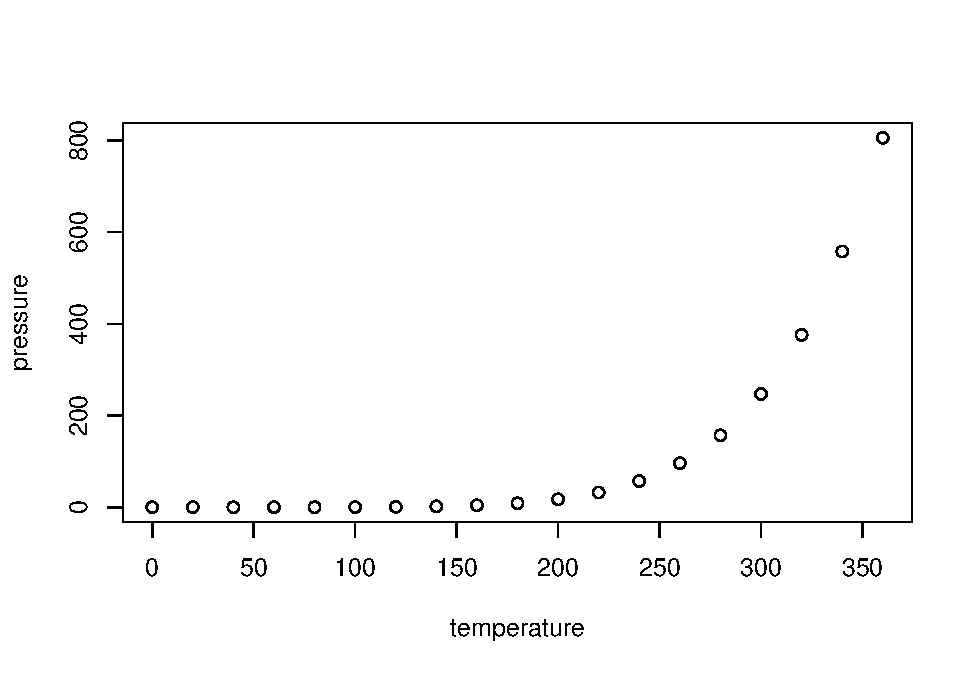
\includegraphics{thesis_files/figure-latex/pressure-1.pdf}

Note that the \texttt{echo\ =\ FALSE} parameter was added to the code chunk to prevent printing of the R code that generated the plot.

\hypertarget{service-frequency}{%
\chapter{Service Frequency}\label{service-frequency}}
\begin{center}\rule{0.5\linewidth}{0.5pt}\end{center}

The purpose of analyzing the service frequency of an existing transit system is to ensure that the level of service has adequate space to accommodate the maximum number of on-board passengers along the entire route over a given time period. Using Remix, both inbound and outbound timetable data were extracted to analyze both the weekday and weekend frequencies and fleet size.

To find the service frequency, divide the total operating hours by the number of trips made by the bus which will give you the average time between each buss arrival along the route or at the stop. Keep in mind, frequency and headway are both terms used to describe the time intervals between buses on a particular route or at a specific bus stop. However, they represent this information in slightly different ways. Frequency refers to the number of bus trips or arrivals at a stop within a specific period, often expressed as the number of buses per hour. For example, a bus service with a frequency of 15 minutes means that a bus arrives approximately every 15 minutes at that stop.

It will be calculated as 1/Time Interval. Headway represents the time interval between the departure or arrival of successive buses. It is the actual time that elapses between one bus leaving or arriving and the next bus following it at a particular stop or along a route.

Headway and frequency can be converted in that:

\[
Frequency = 1/Headway
\]

\[
Headway = 1/Frequency
\]
In other words, Frequency is simply just the inverse of the headway.

\[ Frequency = Headway^{-1} \]

When referring to bus service, a higher frequency or shorter headway generally means better service, providing passengers with more options and shorter waiting times between buses.

\hypertarget{frequency-weekday}{%
\section{3.1 Frequency Weekday}\label{frequency-weekday}}

The frequency weekday was analyzed for both inbound and outbound directions by graphing the average frequency of the existing service for certain time intervals. Based on the frequency data patterns observed for both inbound and outbound, the level of frequency was consistent along the entire route over different time periods for all stops. This was the case for 52 Dundas considering there was not much change in the level of service along the route. To represent the frequency weekday for this route, the frequency of the inbound stop Orchard at Pleasant, and the outbound stop Watson's Lane Loop were used as a benchmark. The maximum frequency for both inbound and outbound is 1.67 buses/hr which occurs during both 06:30 -- 09:30 AM and 15:00 -- 18:00 PM peak hours.

\hypertarget{frequency-weekend}{%
\section{3.2 Frequency Weekend}\label{frequency-weekend}}

Currently, Route 52 Dundas is not scheduled to run during weekends, hence the frequency for the weekend is zero. It could be that there is not enough demand or ridership during the weekends for the 52 Dundas area. This could be something to reconsider when reconfiguring the route.

\hypertarget{fleet-size}{%
\section{3.3 Fleet Size}\label{fleet-size}}

The fleet size for Route 52 is 2 buses for both time periods during the Weekday. As Route 52 does not run-on weekends, there are no fleet sizes reported. The maximum fleet is 2 buses. The buses run every 30 minutes so for the first time period, there is one bus per hour and for the second time period, there is one bus every hour and a half.
\begin{verbatim}
                                               X52.Dundas.Lelouche
1                          https://platform.remix.com/map/81daf133
2                                                                 
3                                                 PROJECT SETTINGS
4                                                       Costing by
5                                                                 
6                                                    Calendar days
7                                                    Weekdays / yr
8                                                   Saturdays / yr
9                                                     Sundays / yr
10                                                                
11                                                   Layover rules
12                                               % of trip runtime
13                                     Minimum flat rate (minutes)
14 For each trip, Remix will use whichever of the above is greater
15                                                                
16                                                    SYSTEM STATS
17                                                   Yearly totals
18                                                           Lines
19                                                        Vehicles
20                                                          $ / yr
21                                                      Hours / yr
22                                                 Trip hours / yr
23                                              Layover hours / yr
24                                                 Kilometers / yr
25                                                           Stops
26                                                     Avg m apart
27                                                                
28                                                   Vehicle Types
29                                                             Bus
30                                                                
31                                                  Weekday totals
32                                                        $ / wkdy
33                                                    Hours / wkdy
34                                               Trip hours / wkdy
35                                            Layover hours / wkdy
36                                               Kilometers / wkdy
37                                                                
38                                                 Saturday totals
39                                                         $ / sat
40                                                     Hours / sat
41                                                Trip hours / sat
42                                             Layover hours / sat
43                                                Kilometers / sat
44                                                                
45                                                   Sunday totals
46                                                         $ / sun
47                                                     Hours / sun
48                                                Trip hours / sun
49                                             Layover hours / sun
50                                                Kilometers / sun
51                                                                
52                                                            Line
53                                                 52 Dundas Local
                 X              X.1          X.2                X.3
1                                                                  
2                                                                  
3                                                                  
4     Vehicle type                                                 
5                                                                  
6                                                                  
7              255                                                 
8               55                                                 
9               55                                                 
10                                                                 
11                                                                 
12             10%                                                 
13                                                                 
14                                                                 
15                                                                 
16                                                                 
17                                                                 
18               1                                                 
19               2                                                 
20         145,860                                                 
21           1,459                                                 
22           1,326                                                 
23             133                                                 
24          31,508                                                 
25              35                                                 
26             296                                                 
27                                                                 
28   Vehicle count            Lines       $ / hr $ / hr (Saturdays)
29               2                1       100.00                  0
30                                                                 
31                                                                 
32             572                                                 
33               6                                                 
34               5                                                 
35               1                                                 
36             124                                                 
37                                                                 
38                                                                 
39                                                                 
40                                                                 
41                                                                 
42                                                                 
43                                                                 
44                                                                 
45                                                                 
46                                                                 
47                                                                 
48                                                                 
49                                                                 
50                                                                 
51                                                                 
52 Inbound, A (km) Outbound, A (km) Vehicle type      Vehicle count
53             5.3              5.2          Bus                  2
                X.4             X.5         X.6        X.7             X.8
1                                                                         
2                                                                         
3                                                                         
4                                                                         
5                                                                         
6                                                                         
7                                                                         
8                                                                         
9                                                                         
10                                                                        
11                                                                        
12                                                                        
13                                                                        
14                                                                        
15                                                                        
16                                                                        
17                                                                        
18                                                                        
19                                                                        
20                                                                        
21                                                                        
22                                                                        
23                                                                        
24                                                                        
25                                                                        
26                                                                        
27                                                                        
28 $ / hr (Sundays)          $ / km $ / vehicle Hours / yr Kilometers / yr
29                0               0           0      1,459          31,508
30                                                                        
31                                                                        
32                                                                        
33                                                                        
34                                                                        
35                                                                        
36                                                                        
37                                                                        
38                                                                        
39                                                                        
40                                                                        
41                                                                        
42                                                                        
43                                                                        
44                                                                        
45                                                                        
46                                                                        
47                                                                        
48                                                                        
49                                                                        
50                                                                        
51                                                                        
52       Hours / yr Kilometers / yr      $ / yr                           
53            1,459          31,508     145,860                           
            X.9
1              
2              
3              
4              
5              
6              
7              
8              
9              
10             
11             
12             
13             
14             
15             
16             
17             
18             
19             
20             
21             
22             
23             
24             
25             
26             
27             
28 Total $ / yr
29      145,860
30             
31             
32             
33             
34             
35             
36             
37             
38             
39             
40             
41             
42             
43             
44             
45             
46             
47             
48             
49             
50             
51             
52             
53             
\end{verbatim}
\hypertarget{service-demand-and-evaluation}{%
\chapter{Service Demand and Evaluation}\label{service-demand-and-evaluation}}
\begin{center}\rule{0.5\linewidth}{0.5pt}\end{center}

In this chapter, service demand and evaluation are explored!

\hypertarget{service-demand}{%
\subsection{Service Demand}\label{service-demand}}

Route 52 only runs during the periods of A.M. peak, midday and P.M. peak. Based on this we decided to allocate 34\% to the A.M. peak, 32\% to the midday period and the last 34\% to the P.M. peak. In the data folder, the distribution of boardings at each stop along the route associated with each time period are detailed. From these results, load profile graphs can be generated. This is where the images of the figures should be displayed, however, it was unable to knit.
\begin{verbatim}
                                                                                                                                                                                                                                                                                                                                                                                                                               ID
1                                                                                                                                                                                                                                                                                                                                                                                                                               1
2                                                                                                                                                                                                                                                                                                                                                                                                                               2
3                                                                                                                                                                                                                                                                                                                                                                                                                               3
4                                                                                                                                                                                                                                                                                                                                                                                                                               4
5                                                                                                                                                                                                                                                                                                                                                                                                                               5
6                                                                                                                                                                                                                                                                                                                                                                                                                               6
7                                                                                                                                                                                                                                                                                                                                                                                                                               7
8                                                                                                                                                                                                                                                                                                                                                                                                                               8
9                                                                                                                                                                                                                                                                                                                                                                                                                               9
10                                                                                                                                                                                                                                                                                                                                                                                                                             10
11                                                                                                                                                                                                                                                                                                                                                                                                                             11
12                                                                                                                                                                                                                                                                                                                                                                                                                             12
13                                                                                                                                                                                                                                                                                                                                                                                                                             13
14                                                                                                                                                                                                                                                                                                                                                                                                                             14
15                                                                                                                                                                                                                                                                                                                                                                                                                             15
16                                                                                                                                                                                                                                                                                                                                                                                                                             16
17                                                                                                                                                                                                                                                                                                                                                                                                                             17
18                                                                                                                                                                                                                                                                                                                                                                                                                             18
19                                                                                                                                                                                                                                                                                                                                                                                                                               
20                                                                                                                                                                                                                                                                                                                                                                                                                               
21                                                                                                                                                                                                                                                                                                                                                                                                                               
22                                                                                                                                                                                                                                                                                                                                                                                                                               
23                                                                                                                                                                                                                                                                                                                                                                                                                               
24                                                                                                                                                                                                                                                                                                                                                                                                                               
25                                                                                                                                                                                                                                                                                                                                                                                                                               
26                                                                                                                                                                                                                                                                                                                                                                                                                               
27                                                                                                                                                                                                                                                                                                                                                                                                                               
28                                                                                                                                                                                                                                                                                                                                                                                                                               
29                                                                                                                                                                                                                                                                                                                                                                                                                               
30                                                                                                                                                                                                                                                                                                                                                                                                                               
31                                                                                                                                                                                                                                                                                                                                                                                                                          NOTE:
32 The frequency we found doing the Load Profile Method was found to be the same frequencies as calculated in Service Frequencies. The minimum frequency is 1 bus per hour for all time periods. With this reasoning, we determined that the service currently allocated within each time interval was appropriate. We assumed the desired occupancy of a 40 ft bus which requires 35 passengers and a capacity of 75 passengers.
33                                                                                                                                                                                                                                                                                                                                                                                                                               
34                                                                                                                                                                                                                                                                                                                                                                                                                               
                             Name Distance.to.next.stop..m. Boardings.weekdays
1             ORCHARD at PLEASANT                       382             39.736
2    TURNBULL opposite KINGS GATE                       197              0.845
3   TURNBULL opposite AUTUMN LEAF                       296              5.474
4             TURNBULL at TERRACE                       582              2.181
5  OLD ANCASTER opposite PLEASANT                       443              1.976
6         OLD ANCASTER at DUNDANA                       129              0.569
7         OGILVIE at OLD ANCASTER                       342              5.525
8            OGILVIE at GOVERNORS                       213             31.535
9              GOVERNOR'S at MAIN                       445              9.705
10                 YORK at COOTES                       170             13.897
11                 YORK at HUNTER                       263              4.267
12                 YORK at DONALD                       322              0.990
13                YORK at CAMERON                       503              1.029
14            YORK opposite MCKAY                       162              2.924
15          YORK opposite WATSONS                       251              1.355
16        YORK opposite FIELDGATE                       383              2.904
17                YORK at OLYMPIC                       203              0.176
18              WATSONS LANE LOOP                                        0.000
19                          Total               5.288018069                   
20                                                                            
21                                                                            
22             Desired Occupancy                         35                   
23                      Capacity                         75                   
24                                                                            
25                                                                            
26           Northbound Direction                  Aj/do*L)               Pm/C
27                      A.M. Peak                  0.070176        0.186666667
28                        Mid-Day                  0.066041        0.173333333
29                      P.M. Peak                  0.070176        0.186666667
30                                                                            
31                                                                            
32                                                                            
33                                                                            
34                                                                            
   A.M..Peak Mid.Day   P.M..Peak Aj.A.M..Peakl Aj.Mid.Day Aj.P.M..Peak  X X.1
1         14      13          14         5.348      4.966        5.348 NA  NA
2          0       0           0         0.000      0.000        0.000 NA  NA
3          2       2           2         0.591      0.591        0.591 NA  NA
4          1       1           1         0.582      0.582        0.582 NA  NA
5          1       1           1         0.443      0.443        0.443 NA  NA
6          0       0           0         0.000      0.000        0.000 NA  NA
7          2       2           2         0.685      0.685        0.685 NA  NA
8         11      10          11         2.343      2.130        2.343 NA  NA
9          3       3           3         1.336      1.336        1.336 NA  NA
10         5       4           5         0.852      0.682        0.852 NA  NA
11         1       1           1         0.263      0.263        0.263 NA  NA
12         0       0           0         0.000      0.000        0.000 NA  NA
13         0       0           0         0.000      0.000        0.000 NA  NA
14         1       1           1         0.162      0.162        0.162 NA  NA
15         0       0           0         0.000      0.000        0.000 NA  NA
16         1       1           1         0.383      0.383        0.383 NA  NA
17         0       0           0         0.000      0.000        0.000 NA  NA
18         0       0           0         0.000      0.000        0.000 NA  NA
19                                      12.988     12.223       12.988 NA  NA
20                                          NA         NA           NA NA  NA
21                                          NA         NA           NA NA  NA
22                                          NA         NA           NA NA  NA
23                                          NA         NA           NA NA  NA
24                                          NA         NA           NA NA  NA
25                                          NA         NA           NA NA  NA
26      Fmin      Fj       Scale            NA         NA           NA NA  NA
27         3       3 Appropriate            NA         NA           NA NA  NA
28       5.5     5.5 Appropriate            NA         NA           NA NA  NA
29         3       3 Appropriate            NA         NA           NA NA  NA
30                                          NA         NA           NA NA  NA
31                                          NA         NA           NA NA  NA
32                                          NA         NA           NA NA  NA
33                                          NA         NA           NA NA  NA
34                                          NA         NA           NA NA  NA
   X.2                          X.3          X.4           X.5
1   NA                                                        
2   NA                                                        
3   NA                                                        
4   NA                                                        
5   NA                                                        
6   NA                                                        
7   NA                                                        
8   NA Distribution of time periods Distribution Redistributed
9   NA  Early Morning (04:00-06:30)           3%              
10  NA      A.M. Peak (06:30-09:30)          34%          0.34
11  NA        Mid-Day (09:30-15:00)          18%          0.32
12  NA      P.M. Peak (15:00-18:00)          29%          0.34
13  NA        Evening (18:00-22:00)          12%              
14  NA     Late Night (22:00-04:00)           4%              
15  NA                                      100%              
16  NA                                                        
17  NA                                                        
18  NA                                                        
19  NA                                                        
20  NA                                                        
21  NA                                                        
22  NA                                                        
23  NA                                                        
24  NA                                                        
25  NA                                                        
26  NA                                                        
27  NA                                                        
28  NA                                                        
29  NA                                                        
30  NA                                                        
31  NA                                                        
32  NA                                                        
33  NA                                                        
34  NA                                                        
\end{verbatim}
\begin{verbatim}
   ID
1   1
2   2
3   3
4   4
5   5
6   6
7   7
8   8
9   9
10 10
11 11
12 12
13 13
14 14
15 15
16 16
17 17
18 18
19 19
20 NA
21 NA
22 NA
23 NA
24 NA
25 NA
26 NA
27 NA
28 NA
29 NA
30 NA
                                                                                                                                                                                                                                                                                                                                                                                                                             Name
1                                                                                                                                                                                                                                                                                                                                                                                                               WATSONS LANE LOOP
2                                                                                                                                                                                                                                                                                                                                                                                                                 YORK at OLYMPIC
3                                                                                                                                                                                                                                                                                                                                                                                                               YORK at FIELDGATE
4                                                                                                                                                                                                                                                                                                                                                                                                                 YORK at WATSONS
5                                                                                                                                                                                                                                                                                                                                                                                                                   YORK at MCKAY
6                                                                                                                                                                                                                                                                                                                                                                                                                 YORK at CAMERON
7                                                                                                                                                                                                                                                                                                                                                                                                            YORK opposite CAIRNS
8                                                                                                                                                                                                                                                                                                                                                                                                                 YORK at WILLETT
9                                                                                                                                                                                                                                                                                                                                                                                                                    YORK at KING
10                                                                                                                                                                                                                                                                                                                                                                                                             GOVERNOR'S at MAIN
11                                                                                                                                                                                                                                                                                                                                                                                                           OGILVIE at GOVERNORS
12                                                                                                                                                                                                                                                                                                                                                                                                        OGILVIE at OLD ANCASTER
13                                                                                                                                                                                                                                                                                                                                                                                                        OLD ANCASTER at PIMLICO
14                                                                                                                                                                                                                                                                                                                                                                                                       OLD ANCASTER at PLEASANT
15                                                                                                                                                                                                                                                                                                                                                                                                            PLEASANT at SUNRISE
16                                                                                                                                                                                                                                                                                                                                                                                                 PLEASANT opposite  AUTUMN LEAF
17                                                                                                                                                                                                                                                                                                                                                                                                         PLEASANT at EDENBRIDGE
18                                                                                                                                                                                                                                                                                                                                                                                                       PLEASANT at GREEN MEADOW
19                                                                                                                                                                                                                                                                                                                                                                                                            ORCHARD at PLEASANT
20                                                                                                                                                                                                                                                                                                                                                                                                                          Total
21                                                                                                                                                                                                                                                                                                                                                                                                                               
22                                                                                                                                                                                                                                                                                                                                                                                                           Southbound Direction
23                                                                                                                                                                                                                                                                                                                                                                                                                        AM Peak
24                                                                                                                                                                                                                                                                                                                                                                                                                        Mid-Day
25                                                                                                                                                                                                                                                                                                                                                                                                                        PM Peak
26                                                                                                                                                                                                                                                                                                                                                                                                                               
27                                                                                                                                                                                                                                                                                                                                                                                                                          NOTE:
28 The frequency we found doing the Load Profile Method was found to be the same frequencies as calculated in Service Frequencies. The minimum frequency is 1 bus per hour for all time periods. With this reasoning, we determined that the service currently allocated within each time interval was appropriate. We assumed the desired occupancy of a 40 ft bus which requires 35 passengers and a capacity of 75 passengers.
29                                                                                                                                                                                                                                                                                                                                                                                                                               
30                                                                                                                                                                                                                                                                                                                                                                                                                               
   Distance.to.next.stop..meters.      Boardings.Weekday       A.M..Peak
1                             164                  8.910               3
2                             343                  0.206               0
3                             227                  3.626               1
4                             213                  7.422               3
5                             459                  1.231               0
6                             252                  2.713               1
7                             342                  0.418               0
8                             259                  0.666               0
9                             427                  1.914               1
10                            181                  7.376               3
11                            351                  8.824               3
12                            122                  3.896               1
13                            435                  2.872               1
14                            285                  0.209               0
15                            253                  0.333               0
16                            282                  0.295               0
17                            218                  4.525               2
18                            359                  3.673               1
19                                                 0.439               0
20                          5.171                                       
21                                                                      
22        Load Profile (Aj/(do*L) Maximum Hourly (Pmj/C) F minimum (Fmj)
23                       0.027524                   0.04               3
24                       0.024146                   0.04             5.5
25                       0.027524                   0.04               3
26                                                                      
27                                                                      
28                                                                      
29                                                                      
30                                                                      
   Mid.Day   P.M..Peak Aj.AM.Peak  Aj.Mid.Day.Peak Aj.PM.Peak  X X.1 X.2 X.3
1        3           3      0.491            0.491      0.491 NA  NA  NA  NA
2        0           0      0.000            0.000      0.000 NA  NA  NA  NA
3        1           1      0.227            0.227      0.227 NA  NA  NA  NA
4        2           3      0.639            0.426      0.639 NA  NA  NA  NA
5        0           0      0.000            0.000      0.000 NA  NA  NA  NA
6        1           1      0.252            0.252      0.252 NA  NA  NA  NA
7        0           0      0.000            0.000      0.000 NA  NA  NA  NA
8        0           0      0.000            0.000      0.000 NA  NA  NA  NA
9        1           1      0.427            0.427      0.427 NA  NA  NA  NA
10       2           3      0.542            0.361      0.542 NA  NA  NA  NA
11       3           3      1.052            1.052      1.052 NA  NA  NA  NA
12       1           1      0.122            0.122      0.122 NA  NA  NA  NA
13       1           1      0.435            0.435      0.435 NA  NA  NA  NA
14       0           0      0.000            0.000      0.000 NA  NA  NA  NA
15       0           0      0.000            0.000      0.000 NA  NA  NA  NA
16       0           0      0.000            0.000      0.000 NA  NA  NA  NA
17       1           2      0.436            0.218      0.436 NA  NA  NA  NA
18       1           1      0.359            0.359      0.359 NA  NA  NA  NA
19       0           0      0.000            0.000      0.000 NA  NA  NA  NA
20                          4.982            4.370      4.982 NA  NA  NA  NA
21                             NA                             NA  NA  NA  NA
22      Fj       Scale         NA Design Occupancy         35 NA  NA  NA  NA
23       3 Appropriate         NA         Capacity         75 NA  NA  NA  NA
24     5.5 Appropriate         NA         Min Freq   1 bus/hr NA  NA  NA  NA
25       3 Appropriate         NA                             NA  NA  NA  NA
26                             NA                             NA  NA  NA  NA
27                             NA                             NA  NA  NA  NA
28                             NA                             NA  NA  NA  NA
29                             NA                             NA  NA  NA  NA
30                             NA                             NA  NA  NA  NA
\end{verbatim}
\hypertarget{service-evaluation}{%
\subsection{Service Evaluation}\label{service-evaluation}}

Use the data file labelled ``Load Profile Analysis'' to begin analyzing the how frequency changes throughout the time periods in a day. In order to evaluate the service utilization, the current frequency and the optimal frequency in each direction must be compared. Based on the steps, the results should be as follows.

For the AM/PM peaks, the current frequency is higher than optimal and therefore the allocated service is over-utilized. Ideally the frequency should be decreased to the minimum of 1 bus per hour to save costs and avoid running empty buses. For the mid-day time period the frequency was 0 as no buses were running at the time however by analyzing the data from task 4 and 5 we can see that the frequency can be brought up to the minimum of 1 bus per hour to accommodate the demand for mid-day service.

From the excel file, Load\_Profile\_Analysis, the desired occupancy of the buses operating on 52 Dundas have a desired occupancy of 35 and a capacity of 75 passengers. The total length route will be the summation of all the distances divided by 1000 to get the distance in kilometres.

\[
Total Distance = \sum (Distance To  Stop)/1000
\]

When analyzing the load profiles, setting up the table as such will make it easier to calculate the Frequencies.

For the northbound direction, the frequency we found doing the Load Profile Method was found to be the same frequencies as calculated in Service Frequencies. The minimum frequency is 1 bus per hour for all time periods. With this reasoning, we determined that the service currently allocated within each time interval was appropriate. We assumed the desired occupancy of a 40 ft bus which requires 35 passengers and a capacity of 75 passengers.

For the southbound direction, the frequency we found doing the Load Profile Method was found to be the same frequencies as calculated in Service Frequencies. The minimum frequency is 1 bus per hour for all time periods. With this reasoning, we determined that the service currently allocated within each time interval was appropriate. We assumed the desired occupancy of a 40 ft bus which requires 35 passengers and a capacity of 75 passengers.

This is what the chart will look like for the \textbf{Northbound} direction.

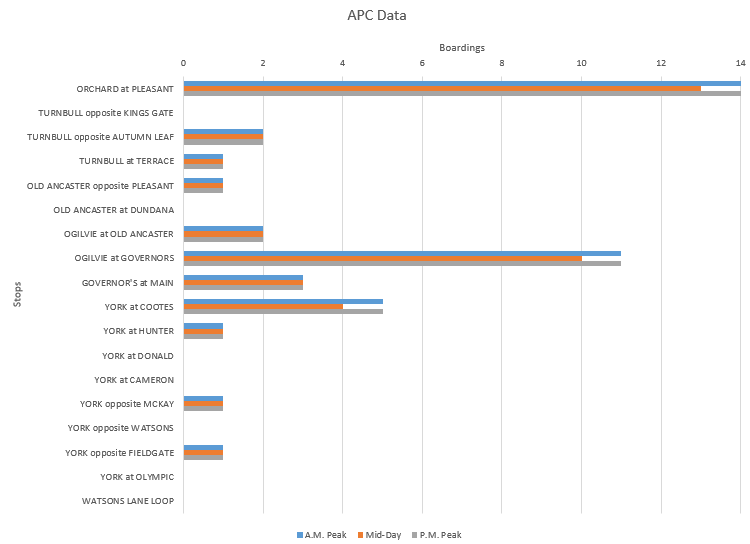
\includegraphics[width=1\linewidth]{figure/Load_Profile_Northbound}

This is what the chart will look like for the \textbf{Southbound} direction.

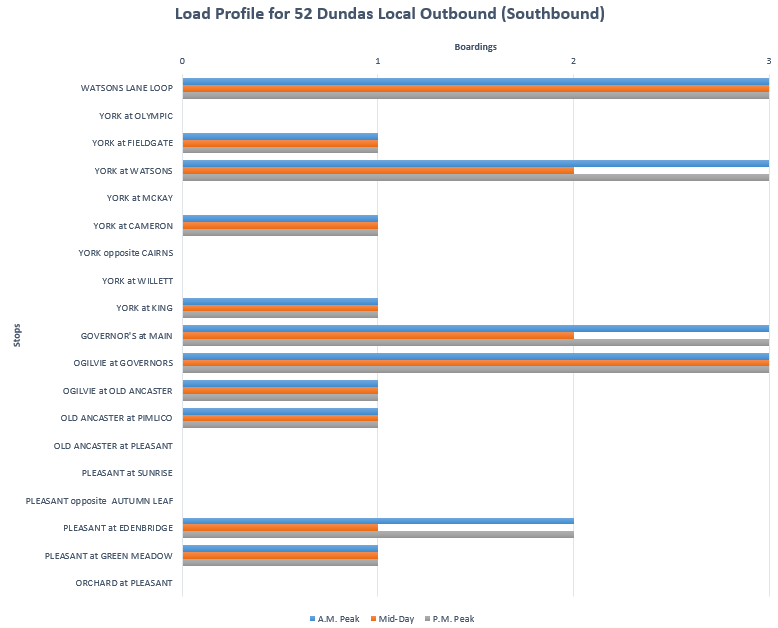
\includegraphics[width=1\linewidth]{figure/Load_Profile_Southbound}

\hypertarget{conclusion}{%
\chapter{Conclusion}\label{conclusion}}
\begin{center}\rule{0.5\linewidth}{0.5pt}\end{center}

A simple analysis was completed for 52 Dundas route in an effort to observe the existing system's infrastructure through changes in operational quality, service quality, and overall connectedness of the transportation grid. From these results, different reconfigurations could be made based on minimizing costs or improving the service within communities in close proximity to the 52 Dundas HSR route. However, it is important to note that there is no perfect, silver-bullet solution for this route or any route for that matter.

The data provided as well as the process of extracting these results have been outlined within this project. File naming, version control with Github, determining the appropriate tools (R Studio and Excel) to use, identifying the infrastructure and then creating a process flow were completed. This project can hopefully be reproduced and repeated with the data and the instructions provided.Ideally, the steps outlined in each of the chapters should allow a user to repeat the steps with the same data provided or alternatively, reproduce similar results with other APC data.

On a personal note, it has been a huge learning experience for me. I have been able to learn many new skills that I did not have at the start of this semester. I came into this course with null knowledge of R and Github and it is amazing what I can now do with the skills I have! Thank you so much Antonio!

\end{document}
